%% Document template source: LaTeX2e template for FEUP's Project FE-UP
%% Document template author: jlopes@fe.up.pt
%% Template adapted

%% A alterar: <--ALTERAR-->

\documentclass[11pt,a4paper]{report}

%% Macros ----------------------------------------------------------------------
\newcommand{\school}{Instituto Superior de Engenharia de Lisboa}
\newcommand{\degree}{Licenciatura em Engenharia Eletrotécnica, Telecomunicações e Computadores}
\newcommand{\projisel}{Projeto ISEL 2023/24 --- LEETC}
\newcommand{\projtitle}{Computer Networks}
\newcommand{\projsubtitle}{Phase 1 - Web Server}
\newcommand{\projteam}{Grupo LP-07}

%% Package ---------------------------------------------------------------------
\usepackage[T1]{fontenc}            % PS fonts
\usepackage[a4paper,left=25mm,right=25mm,top=25mm,bottom=25mm,headheight=6mm,footskip=12mm]{geometry}   % Document dimensions
\usepackage[english]{babel}         % [portuges]??
\usepackage[export]{adjustbox}      %
\usepackage[normalem]{ulem}         % various types of underlining
\usepackage[table,xcdraw]{xcolor}   % driver-independent color extensions
\usepackage[utf8]{inputenc}         % accents
\usepackage{amsmath}                % multi-line and other mathematical statements
\usepackage{array}                  % Images in tables
\usepackage{booktabs}
\usepackage{caption}                % rotating captions, sideways captions, etc.
\usepackage{chicago}                % Bibliography style
\usepackage{color}                  %
\usepackage{fancyhdr}               % Headers and footers
\usepackage{float}                  % tables and figures in the multi-column environment 
\usepackage{graphicx}               % 
\usepackage{hyperref}               % Hyper references
\usepackage{lastpage}               % 
\usepackage{lipsum}                 % loren dummy text
\usepackage{listings}               % Programming syntax
\usepackage{longtable}              % Tables continue in the next page
\usepackage{multicol}               % 
\usepackage{multirow}               % tabular cells spanning multiple rows
\usepackage{newtxtext,newtxmath}    % do not use CM fonts
\usepackage{setspace}               % setting the spacing between lines
\usepackage{subcaption}             % for subfigures and the like

%other macros, if needed
\newcommand{\windspt}{\textsf{WindsPT\/}}
\newcommand{\windscannerpt}{\emph{Windscanner.PT\/}}
\newcommand{\class}[1]{{\normalfont\slshape #1\/}}
\newcommand{\svg}{\class{SVG}}

%environments for infos
\newenvironment{info}[1]{\vspace*{6mm}\color{blue}[ \begin{em} #1}
                        {\vspace*{6mm}\end{em} ]}
\newenvironment{infoopt}[1]{\vspace*{6mm}\color{blue}[ \textbf{Elemento opcional.} \begin{em} #1}
                        {\vspace*{6mm}\end{em} ]}

%% Package settings ------------------------------------------------------------
\graphicspath{{./}}                                 % {graphicx} - Images path
\selectlanguage{portuguese}                         % {babel} - Language portuguese
\setlength{\columnsep}{3cm}                         % {multicol} - Column spacement
\definecolor{engineering}{rgb}{0.549,0.176,0.098}   % {color}
\definecolor{cloudwhite}{cmyk}{0,0,0,0.025}         % {color}
\definecolor{deepblue}{rgb}{0,0,0.5}                % {color}
\definecolor{deepred}{rgb}{0.6,0,0}                 % {color}
\definecolor{deepgreen}{rgb}{0,0.5,0}               % {color}
\setlength{\parindent}{0em}                         % {geometry}
\setlength{\parskip}{1ex}                           % {geometry}
\lstdefinestyle{pythoncode}                         % {listings} - Python syntax
{
    aboveskip=8mm,
    backgroundcolor=\color{cloudwhite},             
    basicstyle=\footnotesize\ttfamily,
    numbers=left,                                   % where to put the line-numbers
    belowskip=4mm,
    breakatwhitespace=false,                        % sets if automatic breaks should only happen at whitespace
    breaklines=true,                                % sets automatic line breaking
    captionpos=b,                                   % sets the caption-position to bottom
    escapeinside={\%*}{*)},                         % if you want to add a comment within your code
    float=htb,
    frame=tb,
    keepspaces=true,
    keywordstyle=\bfseries\color{deepblue},
    morekeywords={*,var,template,new}               % if you want to add more keywords to the set
    numbersep=8pt,                                  % how far the line-numbers are from the code
    numberstyle=\scriptsize\texttt,                 % the size of the fonts that are used for the line-numbers
    showspaces=false,                               % show spaces adding particular underscores
    showstringspaces=false,                         % underline spaces within strings
    showtabs=false,                                 % show tabs within strings adding particular underscores
    stepnumber=1,                                   % the step between two line-numbers. If it's 1 each line will be numbered
    stringstyle=\color{deepgreen},
    tabsize=2,                                      % sets default tabsize to 2 spaces
}
\lstdefinestyle{termoutputs}                        % {listings} - Python syntax
{
    aboveskip=8mm,
    backgroundcolor=\color{cloudwhite},             
    basicstyle=\scriptsize\ttfamily,
    numbers=left,                                   % where to put the line-numbers
    belowskip=4mm,
    breakatwhitespace=false,                        % sets if automatic breaks should only happen at whitespace
    breaklines=true,                                % sets automatic line breaking
    captionpos=b,                                   % sets the caption-position to bottom
    escapeinside={\%*}{*)},                         % if you want to add a comment within your code
    float=htb,
    frame=tb,
    keepspaces=true,
    keywordstyle=\bfseries\color{deepblue},
    morekeywords={*,var,template,new}               % if you want to add more keywords to the set
    numbersep=8pt,                                  % how far the line-numbers are from the code
    numberstyle=\scriptsize\texttt,                 % the size of the fonts that are used for the line-numbers
    showspaces=false,                               % show spaces adding particular underscores
    showstringspaces=false,                         % underline spaces within strings
    showtabs=false,                                 % show tabs within strings adding particular underscores
    stepnumber=1,                                   % the step between two line-numbers. If it's 1 each line will be numbered
    stringstyle=\color{deepgreen},
    tabsize=2,                                      % sets default tabsize to 2 spaces
}
\fancyhf{}                                          % {fancyhdr} clear off all default fancyhdr headers and footers
\lfoot{\small{\emph{\projtitle, \projsubtitle}}}    % {fancyhdr}
\rfoot{\small{\thepage\ / \pageref{LastPage}}}      % {fancyhdr}
\pagestyle{fancy}                                   % {fancyhdr} apply the fancy header style
\renewcommand{\headrulewidth}{0.0pt}                % {fancyhdr} no head rule
\renewcommand{\footrulewidth}{0.4pt}                % {fancyhdr}
\hypersetup{                                        % {hyperref}
    plainpages=false,
    pdfpagelayout=SinglePage,
    bookmarksopen=false,
    bookmarksnumbered=true,
    breaklinks=true,
    linktocpage,
    colorlinks=true,
    linkcolor=engineering,
    urlcolor=engineering,
    filecolor=engineering,
    citecolor=engineering,
    allcolors=engineering
}

%% Document start --------------------------------------------------------------
\begin{document}
\pagenumbering{roman}\setcounter{page}{1}

%% Cover -----------------------------------------------------------------------
\begin{titlepage}
    \center

    \vspace*{-12mm}
    {\large \textbf{\textsc{\school}}}\\

    \vfill

    
\includegraphics[width=62mm]{phase1/images/logoisel}
    
    \vfill
    
    {\huge \textbf{\projtitle}}\\[6mm]
    {\Large \textbf{\projsubtitle}}\\
    
    \vfill
    
    \vfill
    
    {\Large \textbf{\projisel}}\\[12mm]
    
    {\Large \textbf{Coordination}}\\[4mm]
    {\large General: Carlos Meneses\hspace*{18mm}
            Course: Nuno Cruz}\\[6mm]
    
    {\Large \textbf{\projteam}}\\[4mm]
    {\large Supervisor: Luís Pires\hspace*{12mm}}\\[6mm]
    
    {\Large \textbf{Student}}\\[4mm]
    {\large Nuno Brito $<$A46948@alunos.isel.pt$>$}
    
    \vspace*{10mm}
    
    \renewcommand{\today}{April 14th 2024}
    \today
    
\end{titlepage}

%% TOC -------------------------------------------------------------------------
\tableofcontents

%% List of figures -------------------------------------------------------------
\listoffigures
\addcontentsline{toc}{chapter}{Figure list}

%% List of tables --------------------------------------------------------------
\listoftables
\addcontentsline{toc}{chapter}{Table list}

%% List of listings --------------------------------------------------------------
\lstlistoflistings
\addcontentsline{toc}{chapter}{Listings list}

%% Acronyms --------------------------------------------------------------------
\chapter*{Acronyms list}
    \addcontentsline{toc}{chapter}{Acronyms list}

    \begin{flushleft}
        \begin{tabular}{l p{0.8\linewidth}}
            API     & Application Programming Interface\\
            CLI     & Command Line Interface\\
            CMD     & Command Line Prompt\\
            GUI     & Graphical User Interface\\
            HTTP    & Hyper Text Transfer Protocol\\
            HTTPS   & Hyper Text Transfer Protocol Secure\\
            IP      & Internet Protocol\\
            LAN     & Local Area Network\\
            OS      & Operating System\\
            OSS     & openSUSE\\
            PC      & Personal Computer\\
            PHP     & PHP: Hypertext Preprocessor\\
            SSL     & Secure Sockets Layer\\
            TCP     & Transmission Control Protocol\\
            TLS     & Transport Layer Security\\
            TUI     & Terminal User Interface\\ % Not used yet
            UDP     & User Datagram Protocol\\
            VPN     & Virtual Private Network\\
            WWW     & World Wide Web\\
            XAMPP   & Cross-Platform, Apache, MySQL, PHP, and Perl
        \end{tabular}
    \end{flushleft}

%% Glossary --------------------------------------------------------------------
\chapter*{Glossary}
    \addcontentsline{toc}{chapter}{Glossary}

    \begin{description}
        \item[Apache2] \hfill \\
            An opensource HTTP web server.
        \item[Broadcast] \hfill \\
            %TODO
        \item[Browser] \hfill \\
            A browser is a internet navigation software. It comes in multiple flavours, nowadays the big three are Microsoft Edge, Mozilla Firefox and Google Chrome.
        \item[Cisco Packet Tracer] \hfill \\
            %TODO
        \item[Command Line Prompt] \hfill \\
            %TODO
        \item[Firewall] \hfill \\
            A barrier between networks. Controls inbound and outbound traffic.
        \item[Gateway] \hfill \\
            %TODO
        \item[LibreWolf] \hfill \\
            An internet browser based on Mozilla's Firefox. It's primary purpose is to allow privacy, and with it comes security. It achieves this by removing telemetry and data collection.
        \item[Linux] \hfill \\
            %TODO
        \item[MariaDB] \hfill \\
            A community-developed fork of MySQL database server.
        \item[Network] \hfill \\
        \item[openSUSE Tumbleweed] \hfill \\
            An openSUSE (OSS) is an open-source community driven Linux-based distribuition sponsored by SUSE Software Solutions. Tumbleweed is a rolling release version allowing for up-to-date software releases.
        \item[Operating system] \hfill \\
            A program that manages a computer's resources from software to hardware.
        \item[Ping] \hfill \\
            %TODO
        \item[Tracert] \hfill \\
            %TODO
        \item[Ipconfig] \hfill \\
            %TODO
        \item[Python] \hfill \\
            Python is a high-level programming language, object-oriented.
        \item[Perl] \hfill \\
            A high-level, general-purpose, interpreted, dynamic programming language
        \item[Rolling release distribuition] \hfill \\
            A distribuition where it's software release cycle is more frequent than those of Long Term Support (LTS). It's up to the Linux-based distribuitor to guarantee the testing of a package.
        \item[Router] \hfill \\
            %TODO
        \item[Switch] \hfill \\
            %TODO
        \item[Socket] \hfill \\
            A network socket serves as an endpoint for sending and receiving data across the network.
        \item[Subnet Mask] \hfill \\
            %TODO
        \item[Unix] \hfill \\
            %TODO
        \item[VPN] \hfill \\
            A private network creating a secure connection between a device and a network.
        \item[Windows] \hfill \\
            Microsoft's operating system. First released in 1985 as a Graphical User Interface (GUI) for MS-DOS, continued to evolve with it's latest version being 11.
            Due to it's nature, it's not recommended for server production environment.
        \item[Wireshark] \hfill \\
            Wireshark is a network protocol analyser software. Allows traffic capture between a computer and a network.
        \item[XAMPP] \hfill \\
            A software package environment collection containing Apache2 webserver, MariaDB database, PHP and Perl.
    \end{description}

%% Chapter: introduction -------------------------------------------------------
\chapter{Introduction}
% display headers & footers
    \pagestyle{fancy}
    The project consists in building a computer network through four phases. First with a webserver, then simulating a local area network (LAN) with two computers and a switch.
    By the end of the journey, this project will develop into something similar to a corporate network.

    %TODO

% main page numbers with arabic numerals
    \pagenumbering{arabic}\setcounter{page}{1}

%% Chapter: phase 1 ------------------------------------------------------------
\chapter{Phase 1}
%% Chapter: phase 2 ------------------------------------------------------------
\chapter{Phase 2}
%TODO: IP datagram definitions and other stuff
    \section{Connecting two devices with a switch}
        This first part is very simple. There are two devices (PC0 and Laptop0) connected to a switch and their network starts with 192.168.\textbf{\textit{GROUP NUMBER}}.0.\\
        Therefore:

        \begin{itemize}
            \item Group: 7 [192.168.7.0/24]
            \item Laptop0  [192.168.7.1]
            \item PC0      [192.168.7.2]
        \end{itemize}

        After applying the configuration we must run a set of commands to test our network.
        \begin{itemize}
            \item Ping: to test connectivity between devices over IP.
            \item Tracert: diagnostic command for displaying possible routes, also measures transit delay of packages across IP.
            \item Ipconfig: console application program of some computer operating systems that displays all current TCP/IP network configuration values. Unix and linux equivalent is \textit{ifconfig}.
        \end{itemize}

    \subsection{Simulating a network using Cisco Packet Tracer}
        For this project Cisco Packet Tracer will be our main tool. Using the Command Line Prompt (CMD) in each device, will simulate all referenced commands in the network.\\
        So let's get in this magnificient world starting with these steps:\\
        \begin{flushleft}
                \begin{center}
                    \begin{longtable}{ m{5cm} l }
                        \textbf{Steps} & \textbf{Example} \\
                        \hline
                        \endfirsthead
                        \multicolumn{2}{c}%
                        {{\bfseries Table \thetable\ continued from previous page}} \\
                        %{{\bfseries \tablename\ \thetable{} -- continued}} \\
                        \textbf{Steps} & \textbf{Example} \\
                        \hline
                        \endhead
                        \hline Continued on next page \\
                        \endfoot
                        \endlastfoot

                        To configure the IP on a device we must \textbf{single-click} in the intended device (1), go to the \textit{desktop tab} (2) and select \textit{IP Configuration} (3).                                                                                                      & 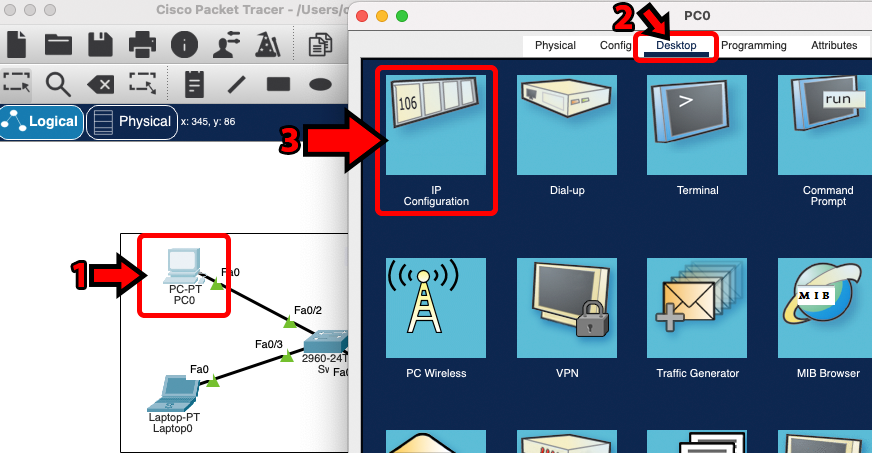
\includegraphics[scale=0.35,valign=c]{phase2/images/p1-connectingdevices/CiscoPacketTracer_configIP} \\ \hline
                        Now we configure our devices according to the required addresses.                                                                                                                                                                                                           & 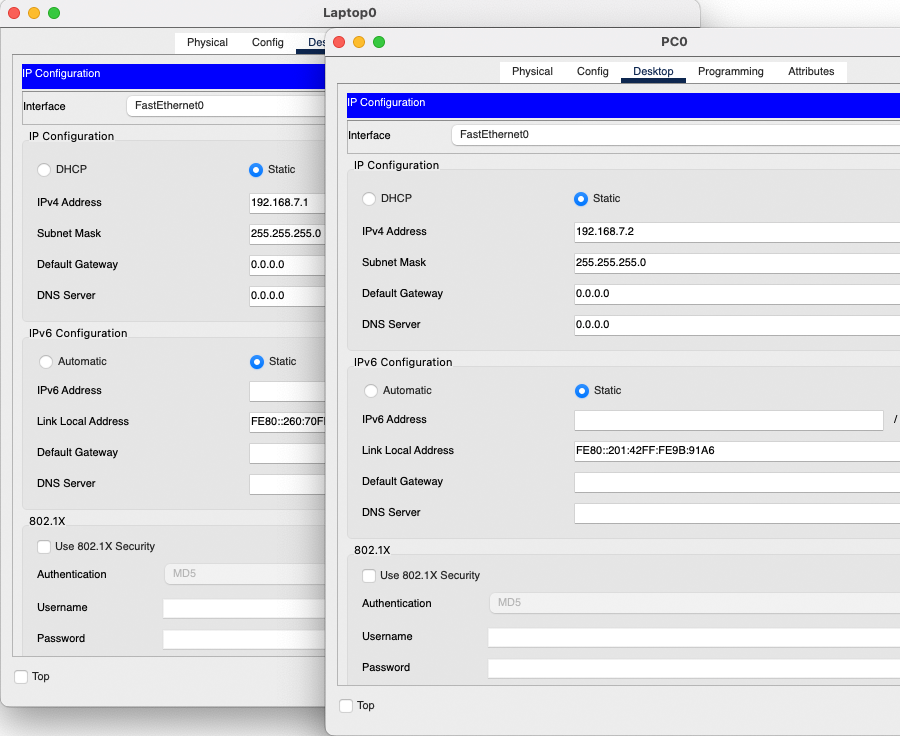
\includegraphics[scale=0.34,valign=c]{phase2/images/p1-connectingdevices/Laptop0PC0_ip} \\ \hline
                        To test the connection we select a device by \textbf{single-clicking} it (1), go to the \textit{desktop tab} (2) and select \textit{Command Prompt} (3).                                                                                                                    & 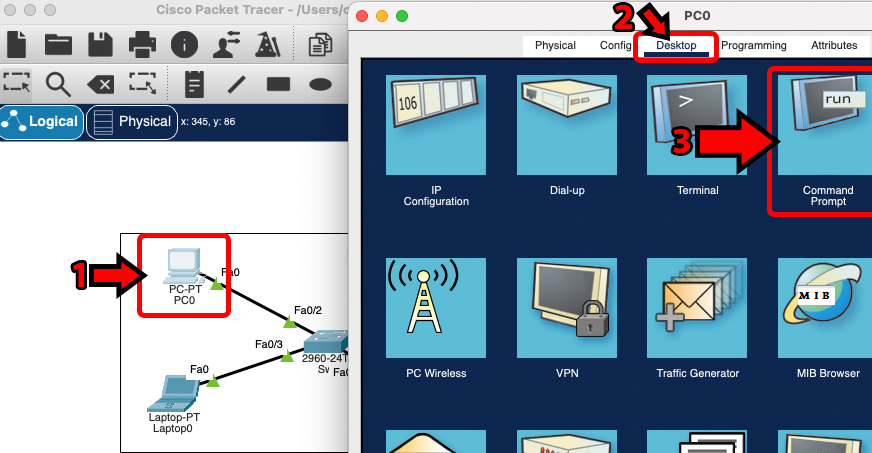
\includegraphics[scale=0.35,valign=c]{phase2/images/p1-connectingdevices/CiscoPacketTracer_cmdOutput} \\ \hline
                        We start by running \textit{arp -a} command, no prior discovery was made so the arp table will be empty. Then will \textit{ping} our other device. Run the \textit{arp -a} command again and will see it populated. If we do a \textit{tracert} there won't be any hops.    & 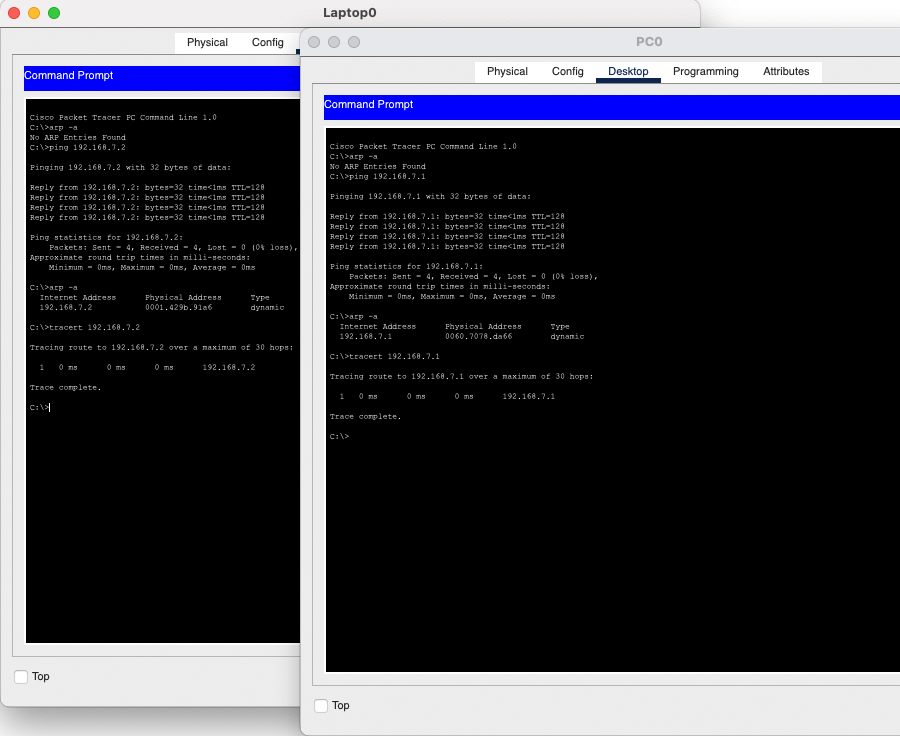
\includegraphics[scale=0.34,valign=c]{phase2/images/p1-connectingdevices/Laptop0PC0_cmd} \\ \hline

                        \caption{Cisco Packet Tracer guide} \label{tab:cptg}
                    \end{longtable}
                \end{center}
        \end{flushleft}

        And to supplement the output images, below are the text versions:
        \lstset{style=termoutputs}
        \lstinputlisting[
            language={},
            caption={PC0 CMD output},
            label={lst:pc0cmdoutp1}
        ]{phase2/outputs/p1-connectingdevices/PC0.txt}
        \lstinputlisting[
            language={},
            caption={Laptop0 CMD output},
            label={lst:laptop0cmdoutp1}
        ]{phase2/outputs/p1-connectingdevices/Laptop0.txt}

        \textbf{Question:} How can a PC know if it is connected to a switch? Is traceroute useful in this situation? \\
        \textbf{Answer:}\\
        \hspace*{10mm}If a device is connected to a switch, the arp table will include both devices IP addresses after a ping to each other. However, if connected to a router (as will see in the next section), they will only include their gateways IP addresses.\\
        \hspace*{10mm}Traceroute isn't very useful here. It only shows hops in a routed network path (layer 3). Layer 2 devices such as switches won't show up since they receive and forward ethernet frames.\\

    \section{Connecting two LANs with a router}
        \lstinputlisting[
            language={},
            numbers=none,
            caption={Network plan},
            label={lst:netplan}
        ]{phase2/outputs/diagram.txt}

        \begin{center}
            \begin{longtable}{rlcccccccccccccccc}
                \hline
                \multicolumn{1}{c}{}                                                                                     & \textbf{}             & \multicolumn{16}{c}{\textbf{IP}}                                                                                                                                                                                                                                                                                                                                                                                                                                                                                  \\ \cline{3-18} 
                \multicolumn{1}{c}{\multirow{-2}{*}{\textbf{Subnet}}}                                                    &                       & \cellcolor[HTML]{C09FE5}0 & \cellcolor[HTML]{C09FE5}3 & \cellcolor[HTML]{C09FE5}4 & \cellcolor[HTML]{C09FE5}7 & \cellcolor[HTML]{C09FE5}8 & \cellcolor[HTML]{C09FE5}11 & \cellcolor[HTML]{C09FE5}12 & \cellcolor[HTML]{C09FE5}15 & \cellcolor[HTML]{BFBFBF}16      & \cellcolor[HTML]{BFBFBF}31      & \cellcolor[HTML]{FFD966}32      & \cellcolor[HTML]{FFD966}63      & \cellcolor[HTML]{A9D08E}64      & \cellcolor[HTML]{A9D08E}127     & \cellcolor[HTML]{F4B084}128      & \cellcolor[HTML]{F4B084}255     \\ \cline{1-1} \cline{3-18} 
                \endfirsthead
                %
                \multicolumn{18}{c}%
                {{\bfseries Table \thetable\ continued from previous page}} \\
                \hline
                \multicolumn{1}{c}{}                                                                                     & \textbf{}             & \multicolumn{16}{c}{\textbf{IP}}                                                                                                                                                                                                                                                                                                                                                                                                                                                                                  \\ \cline{3-18} 
                \multicolumn{1}{c}{\multirow{-2}{*}{\textbf{Subnet}}}                                                    &                       & \cellcolor[HTML]{C09FE5}0 & \cellcolor[HTML]{C09FE5}3 & \cellcolor[HTML]{C09FE5}4 & \cellcolor[HTML]{C09FE5}7 & \cellcolor[HTML]{C09FE5}8 & \cellcolor[HTML]{C09FE5}11 & \cellcolor[HTML]{C09FE5}12 & \cellcolor[HTML]{C09FE5}15 & \cellcolor[HTML]{BFBFBF}16      & \cellcolor[HTML]{BFBFBF}31      & \cellcolor[HTML]{FFD966}32      & \cellcolor[HTML]{FFD966}63      & \cellcolor[HTML]{A9D08E}64      & \cellcolor[HTML]{A9D08E}127     & \cellcolor[HTML]{F4B084}128      & \cellcolor[HTML]{F4B084}255     \\ \cline{1-1} \cline{3-18} 
                \endhead
                %
                \cline{1-1} \cline{3-18}
                \endfoot
                %
                \endlastfoot
                %
                \textbf{/25}                                                                                             &                       &                           &                           &                           &                           &                           &                            &                            &                            &                                 &                                 &                                 &                                 &                                 &                                 & \cellcolor[HTML]{F4B084}         & \cellcolor[HTML]{F4B084}        \\
                \textbf{/26}                                                                                             &                       &                           &                           &                           &                           &                           &                            &                            &                            &                                 &                                 &                                 &                                 & \cellcolor[HTML]{A9D08E}        & \cellcolor[HTML]{A9D08E}        &                                  &                                 \\
                \textbf{/27}                                                                                             &                       &                           &                           &                           &                           &                           &                            &                            &                            &                                 &                                 & \cellcolor[HTML]{FFD966}        & \cellcolor[HTML]{FFD966}        &                                 &                                 &                                  &                                 \\
                \textbf{/28}                                                                                             &                       &                           &                           &                           &                           &                           &                            &                            &                            & \cellcolor[HTML]{BFBFBF}        & \cellcolor[HTML]{BFBFBF}        &                                 &                                 &                                 &                                 &                                  &                                 \\
                \textbf{/30}                                                                                             &                       &                           &                           &                           &                           &                           &                            & \cellcolor[HTML]{C09FE5}   & \cellcolor[HTML]{C09FE5}   &                                 &                                 &                                 &                                 &                                 &                                 &                                  &                                 \\
                \textbf{/30}                                                                                             &                       &                           &                           &                           &                           & \cellcolor[HTML]{C09FE5}  & \cellcolor[HTML]{C09FE5}   &                            &                            &                                 &                                 &                                 &                                 &                                 &                                 &                                  &                                 \\
                \textbf{/30}                                                                                             &                       &                           &                           & \cellcolor[HTML]{C09FE5}  & \cellcolor[HTML]{C09FE5}  &                           &                            &                            &                            &                                 &                                 &                                 &                                 &                                 &                                 &                                  &                                 \\
                \textbf{/30}                                                                                             &                       & \cellcolor[HTML]{C09FE5}  & \cellcolor[HTML]{C09FE5}  &                           &                           &                           &                            &                            &                            &                                 &                                 &                                 &                                 &                                 &                                 &                                  &                                 \\ \cline{1-1} \cline{3-18} 
                                                                                                                         & \multicolumn{1}{l|}{} & \multicolumn{2}{l}{\cellcolor[HTML]{C09FE5}/30}       & \multicolumn{2}{c}{\cellcolor[HTML]{C09FE5}/30}       & \multicolumn{2}{c}{\cellcolor[HTML]{C09FE5}/30}        & \multicolumn{2}{c}{\cellcolor[HTML]{C09FE5}/30}         & \multicolumn{2}{c}{\cellcolor[HTML]{BFBFBF}}                      & \multicolumn{2}{c}{\cellcolor[HTML]{FFD966}}                      & \multicolumn{2}{c}{\cellcolor[HTML]{A9D08E}}                      & \multicolumn{2}{c|}{\cellcolor[HTML]{F4B084}}                      \\
                                                                                                                         & \multicolumn{1}{l|}{} & \multicolumn{4}{l}{/29}                                                                                       & \multicolumn{4}{c}{}                                                                                             & \multicolumn{2}{c}{\cellcolor[HTML]{BFBFBF}}                      & \multicolumn{2}{c}{\cellcolor[HTML]{FFD966}}                      & \multicolumn{2}{c}{\cellcolor[HTML]{A9D08E}}                      & \multicolumn{2}{c|}{\cellcolor[HTML]{F4B084}}                      \\
                                                                                                                         & \multicolumn{1}{l|}{} & \multicolumn{8}{l}{\cellcolor[HTML]{BFBFBF}/28}                                                                                                                                                                                  & \multicolumn{2}{c}{\multirow{-3}{*}{\cellcolor[HTML]{BFBFBF}/28}} & \multicolumn{2}{c}{\cellcolor[HTML]{FFD966}}                      & \multicolumn{2}{c}{\cellcolor[HTML]{A9D08E}}                      & \multicolumn{2}{c|}{\cellcolor[HTML]{F4B084}}                      \\
                                                                                                                         & \multicolumn{1}{l|}{} & \multicolumn{10}{l}{\cellcolor[HTML]{FFD966}/27}                                                                                                                                                                                                                                                     & \multicolumn{2}{c}{\multirow{-4}{*}{\cellcolor[HTML]{FFD966}/27}} & \multicolumn{2}{c}{\cellcolor[HTML]{A9D08E}}                      & \multicolumn{2}{c|}{\cellcolor[HTML]{F4B084}}                      \\
                                                                                                                         & \multicolumn{1}{l|}{} & \multicolumn{12}{l}{\cellcolor[HTML]{A9D08E}/26}                                                                                                                                                                                                                                                                                                                         & \multicolumn{2}{c}{\multirow{-5}{*}{\cellcolor[HTML]{A9D08E}/26}} & \multicolumn{2}{c|}{\cellcolor[HTML]{F4B084}}                      \\
                                                                                                                         & \multicolumn{1}{l|}{} & \multicolumn{14}{l}{\cellcolor[HTML]{F4B084}/25}                                                                                                                                                                                                                                                                                                                                                                                             & \multicolumn{2}{c|}{\multirow{-6}{*}{\cellcolor[HTML]{F4B084}/25}} \\
                \multirow{-7}{*}{\textbf{\begin{tabular}[c]{@{}r@{}}Subnet\\      visual\\      portrayal\end{tabular}}} & \multicolumn{1}{l|}{} & \multicolumn{16}{l|}{\cellcolor[HTML]{00B0F0}/24}                                                                                                                                                                                                                                                                                                                                                                                                                                                                 \\ \cline{1-1} \cline{3-18} 
                \caption{Visual LAN allocation}
                \label{tab:visuallanalloc}\\
            \end{longtable}
        \end{center}

        \begin{center}
            \begin{longtable}{lllllll}
                \hline
                                                               & \textbf{Network}           & \textbf{Usable IPs} & \textbf{Router} & \multicolumn{1}{c}{\textbf{Broadcast}} & \multicolumn{1}{c}{\textbf{Subnet Mask}} &                                      \\ \cline{2-6}
                \multirow{-2}{*}{\textbf{Name}}                & \multicolumn{5}{c}{192.168.7.}                                                                                                                         & \multirow{-2}{*}{\textbf{Populated}} \\ \hline
                \endfirsthead
                %
                \multicolumn{7}{c}%
                {{\bfseries Table \thetable\ continued from previous page}} \\
                \hline
                                                               & \textbf{Network}           & \textbf{Usable IPs} & \textbf{Router} & \multicolumn{1}{c}{\textbf{Broadcast}} & \multicolumn{1}{c}{\textbf{Subnet Mask}} &                                      \\ \cline{2-6}
                \multirow{-2}{*}{\textbf{Name}}                & \multicolumn{5}{c}{192.168.7.}                                                                                                                         & \multirow{-2}{*}{\textbf{Populated}} \\ \hline
                \endhead
                %
                \hline
                \endfoot
                %
                \endlastfoot
                %
                \cellcolor[HTML]{F4B084}\textbf{LAN Server}    & 128                        & 129 - 253           & 254             & 255                                    & 128                                      & 126                                  \\
                \cellcolor[HTML]{A9D08E}\textbf{LAN A}         & 64                         & 65 - 125            & 126             & 127                                    & 192                                      & 48                                   \\
                \cellcolor[HTML]{FFD966}\textbf{LAN B}         & 32                         & 33 - 61             & 62              & 63                                     & 224                                      & 27                                   \\ \hline
                                                               & \cellcolor[HTML]{BFBFBF}16 & 17 - 31             &                 & 32                                     &                                          & 0                                    \\
                \multirow{-2}{*}{\textbf{Unused remaining}}    & \cellcolor[HTML]{C09FE5}12 & 13 - 14             &                 & 15                                     &                                          & 0                                    \\ \hline
                \cellcolor[HTML]{C09FE5}\textbf{LAN Transit C} & 8                          & 9 - 10              &                 & 11                                     & 252                                      & 2                                    \\
                \cellcolor[HTML]{C09FE5}\textbf{LAN Transit B} & 4                          & 5 - 6               &                 & 7                                      & 252                                      & 2                                    \\
                \cellcolor[HTML]{C09FE5}\textbf{LAN Transit A} & 0                          & 1 - 2               &                 & 3                                      & 252                                      & 2                                    \\ \hline
                \caption{LAN allocation table}
                \label{tab:lanalloctable}\\
            \end{longtable}
        \end{center}

        \begin{center}
            \begin{longtable}{@{}llllll@{}}
                \toprule
                \multicolumn{1}{c}{\multirow{2}{*}{\textbf{Name}}} & \multicolumn{1}{c}{\multirow{2}{*}{\textbf{Ports Link}}} & \multicolumn{1}{c}{\multirow{2}{*}{\textbf{Network}}} & \multicolumn{1}{c}{\multirow{2}{*}{\textbf{IP}}} & \multicolumn{1}{c}{\multirow{2}{*}{\textbf{Subnet Mask}}} & \multicolumn{1}{c}{\multirow{2}{*}{\textbf{Gateway}}} \\
                \multicolumn{1}{c}{}                               & \multicolumn{1}{c}{}                                     & \multicolumn{1}{c}{}                                  & \multicolumn{1}{c}{}                             & \multicolumn{1}{c}{}                                      & \multicolumn{1}{c}{}                                  \\* \midrule
                \endfirsthead
                %
                \multicolumn{6}{c}%
                {{\bfseries Table \thetable\ continued from previous page}} \\
                \toprule
                \multicolumn{1}{c}{\multirow{2}{*}{\textbf{Name}}} & \multicolumn{1}{c}{\multirow{2}{*}{\textbf{Ports Link}}} & \multicolumn{1}{c}{\multirow{2}{*}{\textbf{Network}}} & \multicolumn{1}{c}{\multirow{2}{*}{\textbf{IP}}} & \multicolumn{1}{c}{\multirow{2}{*}{\textbf{Subnet Mask}}} & \multicolumn{1}{c}{\multirow{2}{*}{\textbf{Gateway}}} \\
                \multicolumn{1}{c}{}                               & \multicolumn{1}{c}{}                                     & \multicolumn{1}{c}{}                                  & \multicolumn{1}{c}{}                             & \multicolumn{1}{c}{}                                      & \multicolumn{1}{c}{}                                  \\* \midrule
                \endhead
                %
                \bottomrule
                \endfoot
                %
                \endlastfoot
                %
                \textbf{PC0}                                       & Fa0 - Sw0 Fa0/2                                          & \multirow{2}{*}{LAN A}                                & 192.168.7.65                                     & 255.255.255.192                                           & 192.168.7.126                                         \\
                \textbf{Laptop0}                                   & Fa0 - Sw0 Fa0/3                                          &                                                       & 192.168.7.66                                     & 255.255.255.192                                           & 192.168.7.126                                         \\* \midrule
                \textbf{PC1}                                       & Fa0 - Sw1 Fa0/2                                          & \multirow{2}{*}{LAN B}                                & 192.168.7.33                                     & 255.255.255.224                                           & 192.168.7.62                                          \\
                \textbf{Laptop1}                                   & Fa0 - Sw1 Fa0/3                                          &                                                       & 192.168.7.34                                     & 255.255.255.224                                           & 192.168.7.62                                          \\* \midrule
                \multirow{3}{*}{\textbf{R0}}                       & Fa5/0 - R1 Fa5/0                                         & LAN Transit B                                         & 192.168.7.5                                      & 255.255.255.252                                           &                                                       \\
                                                                   & Fa4/0 - R2 Fa4/0                                         & LAN Transit C                                         & 192.168.7.9                                      & 255.255.255.252                                           &                                                       \\
                                                                   & Fa0/0                                                    & External                                              &                                                  &                                                           &                                                       \\* \midrule
                \multirow{4}{*}{\textbf{R1}}                       & Fa4/0 - R2 Fa5/0                                         & LAN Transit A                                         & 192.168.7.1                                      & 255.255.255.252                                           &                                                       \\
                                                                   & Fa5/0 - R1 Fa4/0                                         & LAN Transit B                                         & 192.168.7.6                                      & 255.255.255.252                                           &                                                       \\
                                                                   & Fa0/0 - Sw0 Fa0/1                                        & LAN A                                                 & 192.168.7.126                                    & 255.255.255.192                                           &                                                       \\
                                                                   & Fa1/0 - Sw1 Fa0/1                                        & LAN B                                                 & 192.168.7.62                                     & 255.255.255.224                                           &                                                       \\* \midrule
                \multirow{3}{*}{\textbf{R2}}                       & Fa5/0 - R1 Fa4/0                                         & LAN Transit A                                         & 192.168.7.2                                      & 255.255.255.252                                           &                                                       \\
                                                                   & Fa4/0 - R0 Fa4/0                                         & LAN Transit C                                         & 192.168.7.10                                     & 255.255.255.252                                           &                                                       \\
                                                                   & Fa0/0 - Sw2 Fa0/4                                        & LAN Server                                            & 192.168.7.254                                    & 255.255.255.128                                           &                                                       \\* \midrule
                \textbf{DHCP Server}                               & Fa0 - Sw2 Fa0/3                                          & \multirow{3}{*}{LAN Server}                           & 192.168.7.129                                    & 255.255.255.128                                           & 192.168.7.254                                         \\
                \textbf{DNS Server}                                & Fa0 - Sw2 Fa0/2                                          &                                                       & 192.168.7.130                                    & 255.255.255.128                                           & 192.168.7.254                                         \\
                \textbf{HTTP Server}                               & Fa0 - Sw2 Fa0/1                                          &                                                       & 192.168.7.131                                    & 255.255.255.128                                           & 192.168.7.254                                         \\* \midrule
                \multirow{3}{*}{\textbf{Sw0}}                      & Fa0/1 - R1 Fa0/0                                         & \multirow{3}{*}{LAN A}                                & \multicolumn{1}{c}{}                             & \multicolumn{1}{c}{}                                      & \multicolumn{1}{c}{}                                  \\
                                                                   & Fa0/2 - PC0                                              &                                                       & \multicolumn{1}{c}{}                             & \multicolumn{1}{c}{}                                      & \multicolumn{1}{c}{}                                  \\
                                                                   & Fa0/3 - Laptop0                                          &                                                       & \multicolumn{1}{c}{}                             & \multicolumn{1}{c}{}                                      & \multicolumn{1}{c}{}                                  \\* \midrule
                \multirow{3}{*}{\textbf{Sw1}}                      & Fa0/1 - R1 Fa1/0                                         & \multirow{3}{*}{LAN B}                                & \multicolumn{1}{c}{}                             & \multicolumn{1}{c}{}                                      & \multicolumn{1}{c}{}                                  \\
                                                                   & Fa0/2 - PC1                                              &                                                       & \multicolumn{1}{c}{}                             & \multicolumn{1}{c}{}                                      & \multicolumn{1}{c}{}                                  \\
                                                                   & Fa0/3 - Laptop1                                          &                                                       & \multicolumn{1}{c}{}                             & \multicolumn{1}{c}{}                                      & \multicolumn{1}{c}{}                                  \\* \midrule
                \multirow{4}{*}{\textbf{Sw2}}                      & Fa0/1 - HTTP                                             & \multirow{4}{*}{LAN Server}                           & \multicolumn{1}{c}{}                             & \multicolumn{1}{c}{}                                      & \multicolumn{1}{c}{}                                  \\
                                                                   & Fa0/2 - DNS                                              &                                                       & \multicolumn{1}{c}{}                             & \multicolumn{1}{c}{}                                      & \multicolumn{1}{c}{}                                  \\
                                                                   & Fa0/3 - DHCP                                             &                                                       & \multicolumn{1}{c}{}                             & \multicolumn{1}{c}{}                                      & \multicolumn{1}{c}{}                                  \\
                                                                   & Fa0/4 - R2 Fa0/0                                         &                                                       & \multicolumn{1}{c}{}                             & \multicolumn{1}{c}{}                                      & \multicolumn{1}{c}{}                                  \\* \bottomrule
                \caption{IP configuration table}
                \label{tab:deviceiptable}\\
                \end{longtable}
        \end{center}

        The above tables will be used through out the project. Instead of planning for each phase and re-assigning the entire network, It was opted to fully outline every subnet and device for the sake of simplicity and work.
        However, here we'll focus on router \textbf{\textit{R1}}, and networks \textbf{\textit{LAN A}} and \textbf{\textit{LAN B}}. For now let's just focus on the IP addresses, the meaning of values will be explained in Phase 3.
        And once again, \textbf{Cisco Packet Tracer} to the help:

        \begin{flushleft}
                \begin{center}
                    \begin{longtable}{ m{5cm} l }
                        \textbf{Steps} & \textbf{Example} \\
                        \hline
                        \endfirsthead
                        \multicolumn{2}{c}%
                        {{\bfseries Table \thetable\ continued from previous page}} \\
                        %{{\bfseries \tablename\ \thetable{} -- continued}} \\
                        \textbf{Steps} & \textbf{Example} \\
                        \hline
                        \endhead
                        \hline Continued on next page \\
                        \endfoot
                        \endlastfoot

                        text & 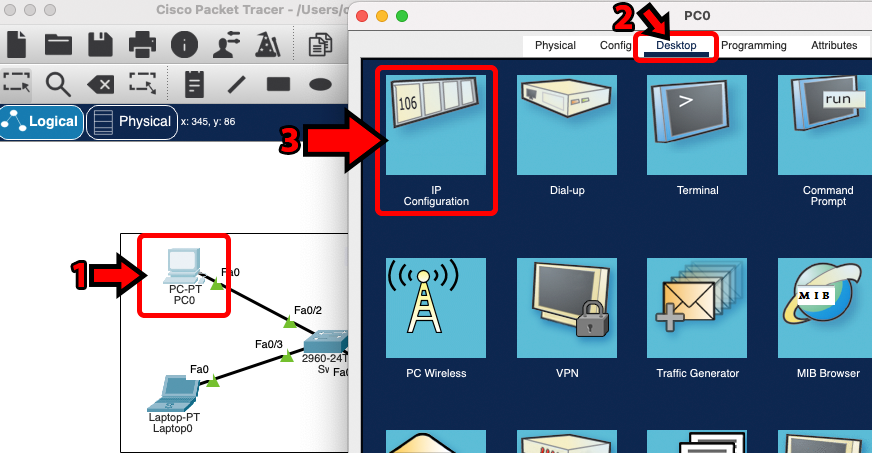
\includegraphics[scale=0.35,valign=c]{phase2/images/p1-connectingdevices/CiscoPacketTracer_configIP} \\ \hline
                        text & 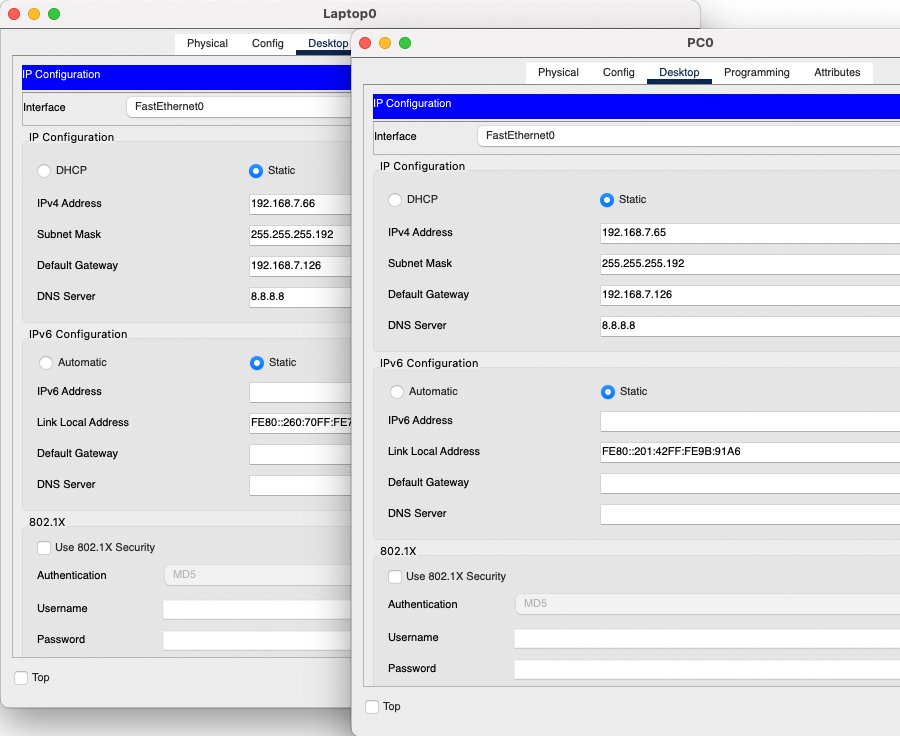
\includegraphics[scale=0.34,valign=c]{phase2/images/p2-connecting2lanswithrouter/Laptop0PC0_ip} \\ \hline
                        text & 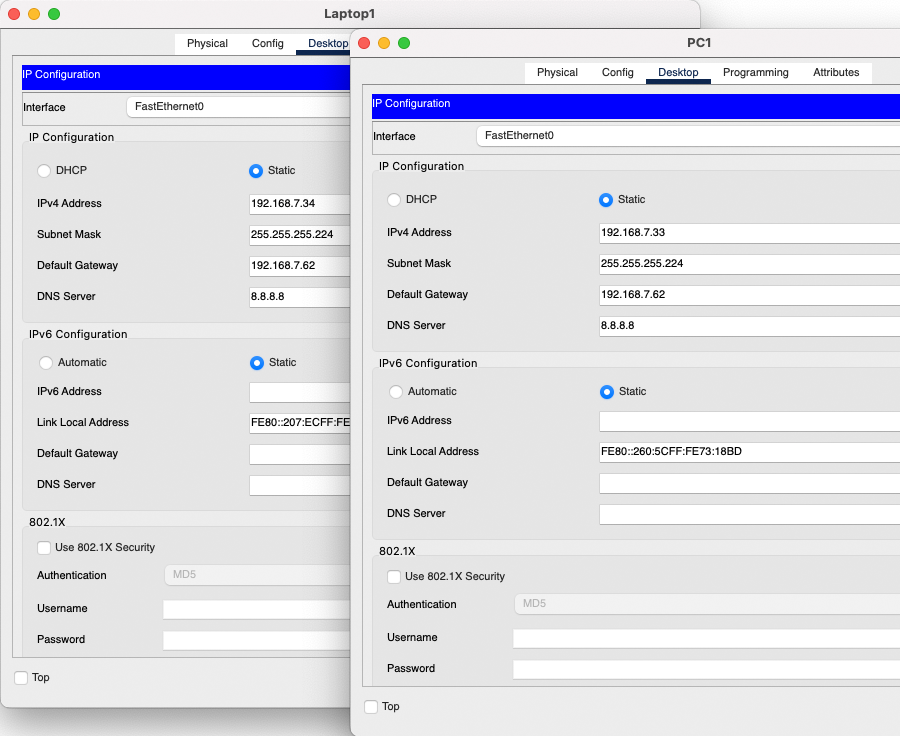
\includegraphics[scale=0.34,valign=c]{phase2/images/p2-connecting2lanswithrouter/Laptop1PC1_ip} \\ \hline
                        text & 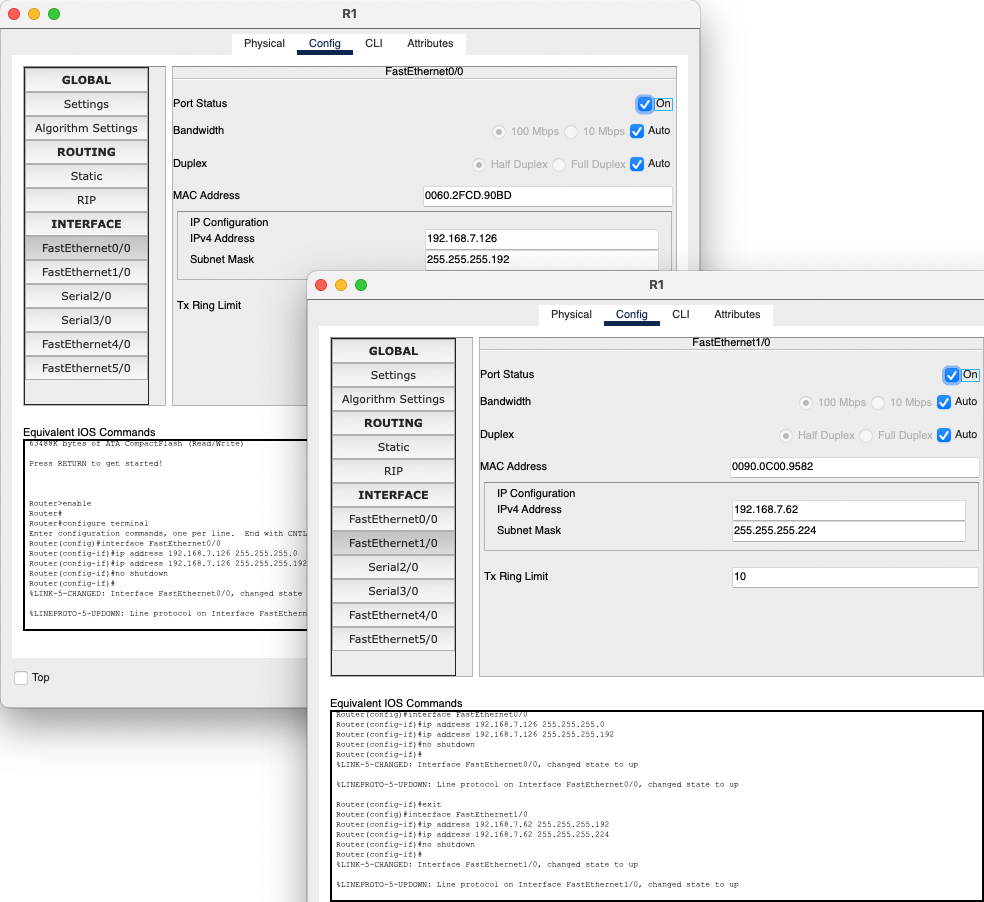
\includegraphics[scale=0.31,valign=c]{phase2/images/p2-connecting2lanswithrouter/R1-interfaces} \\ \hline
                        text & 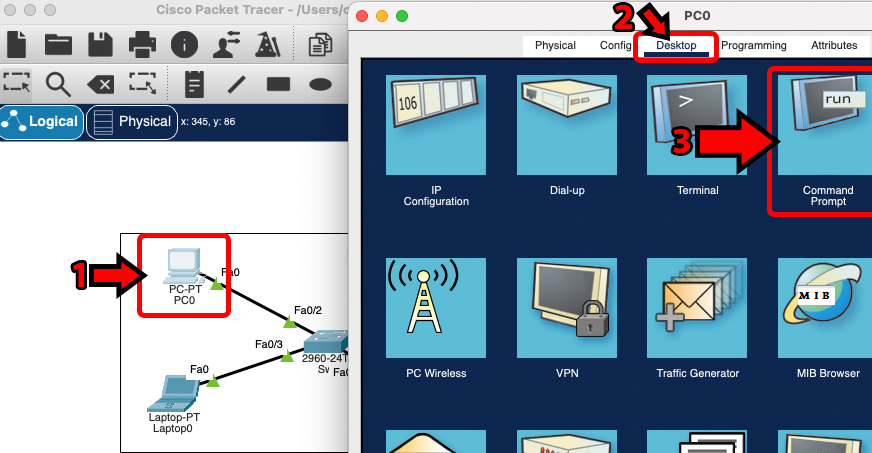
\includegraphics[scale=0.35,valign=c]{phase2/images/p1-connectingdevices/CiscoPacketTracer_cmdOutput} \\ \hline
                        text & 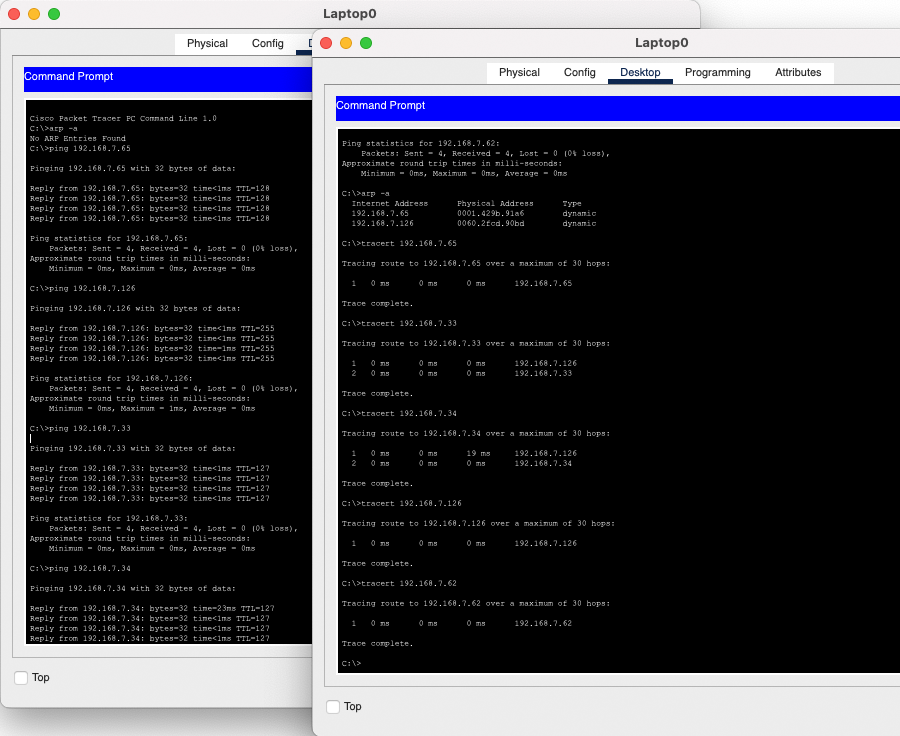
\includegraphics[scale=0.34,valign=c]{phase2/images/p2-connecting2lanswithrouter/Laptop0_cmdall} \\ \hline
                        text & 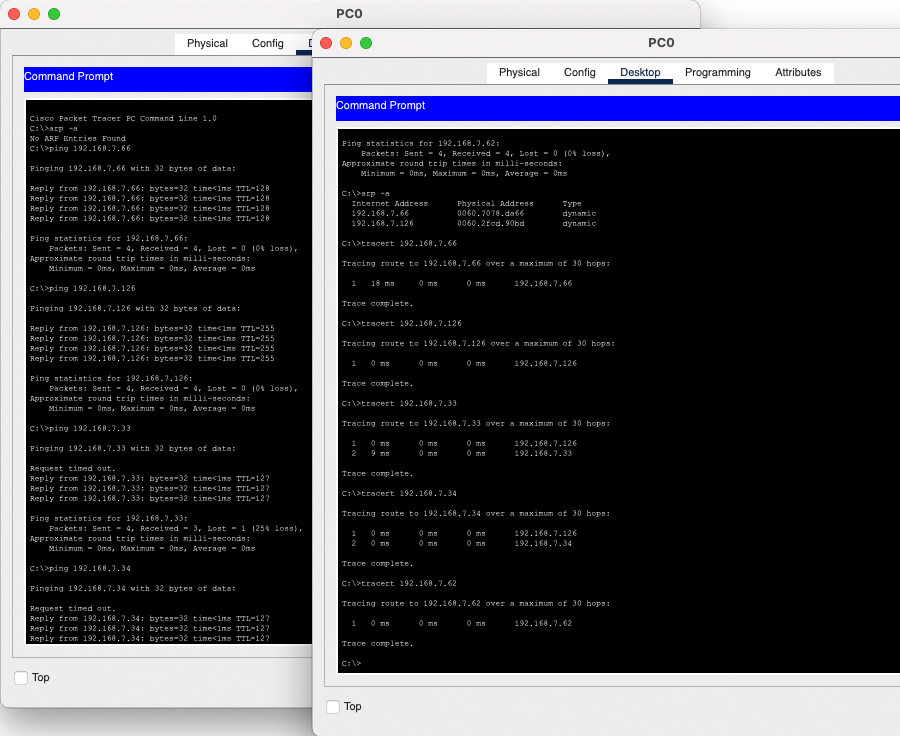
\includegraphics[scale=0.34,valign=c]{phase2/images/p2-connecting2lanswithrouter/PC0_cmdall} \\ \hline
                        text & 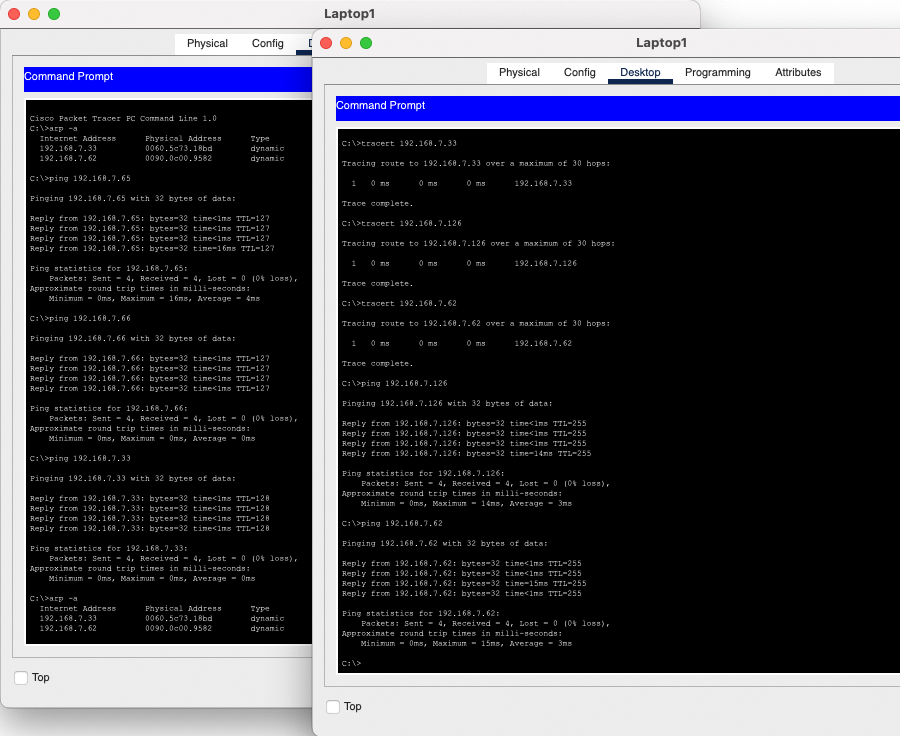
\includegraphics[scale=0.34,valign=c]{phase2/images/p2-connecting2lanswithrouter/Laptop1_cmdall} \\ \hline
                        text & 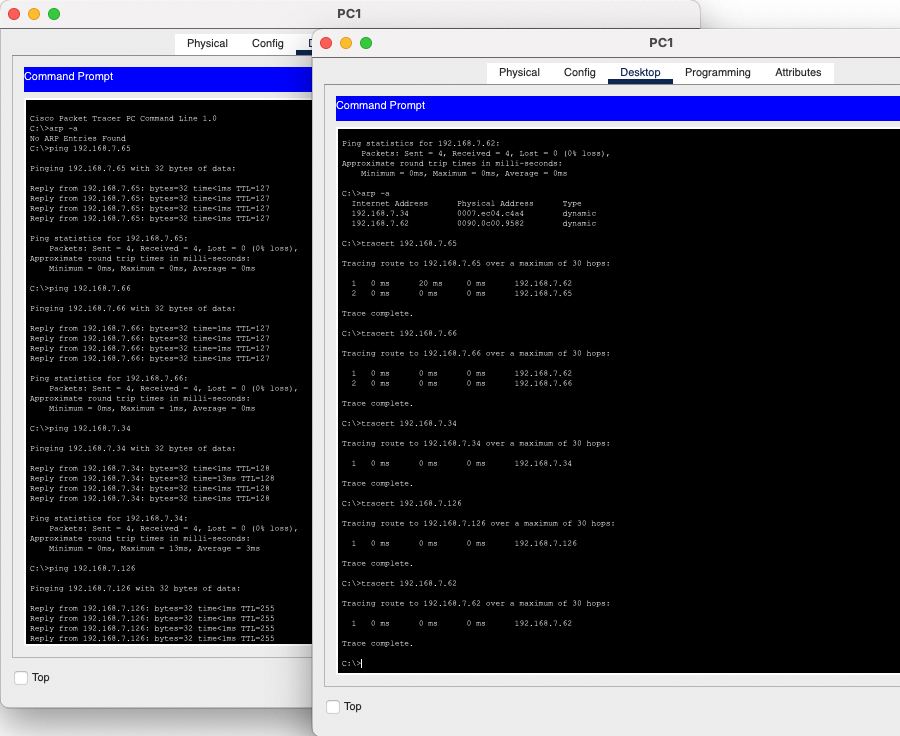
\includegraphics[scale=0.34,valign=c]{phase2/images/p2-connecting2lanswithrouter/PC1_cmdall} \\ \hline
                        text & 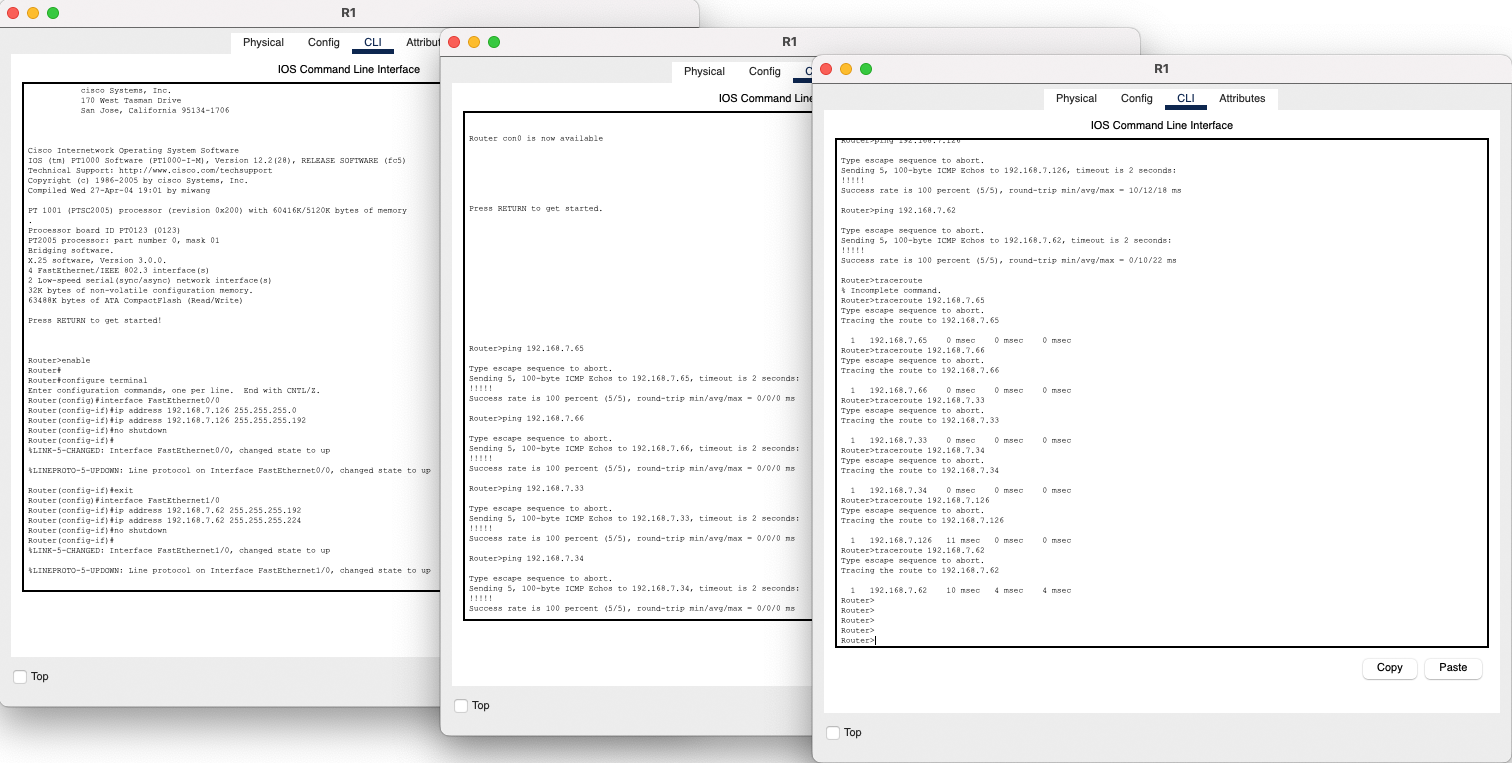
\includegraphics[scale=0.202,valign=c]{phase2/images/p2-connecting2lanswithrouter/R1-cliall} \\ \hline

                        \caption{Cisco Packet Tracer guide} \label{tab:cptg2}
                    \end{longtable}
                \end{center}
        \end{flushleft}

        And to supplement the output images, below are the text versions \textit{(considering this isn't a report for ants)}:
        \lstset{style=termoutputs}
        \lstinputlisting[
            language={},
            caption={PC0 CMD output},
            label={lst:pc0cmdoutp2}
        ]{phase2/outputs/p2-connecting2lanswithrouter/PC0.txt}
        \lstinputlisting[
            language={},
            caption={Laptop0 CMD output},
            label={lst:laptop0cmdoutp2}
        ]{phase2/outputs/p2-connecting2lanswithrouter/Laptop0.txt}
        \lstinputlisting[
            language={},
            caption={PC1 CMD output},
            label={lst:pc1cmdoutp2}
        ]{phase2/outputs/p2-connecting2lanswithrouter/PC1.txt}
        \lstinputlisting[
            language={},
            caption={Laptop1 CMD output},
            label={lst:laptop1cmdoutp2}
        ]{phase2/outputs/p2-connecting2lanswithrouter/Laptop1.txt}
        \lstinputlisting[
            language={},
            caption={Router 1 CLI output},
            label={lst:r1cmdoutp2}
        ]{phase2/outputs/p2-connecting2lanswithrouter/R1.txt}

%% Chapter: recomendations -----------------------------------------------------
\chapter{Issues and fixes}
    Running python code: \\
        \hspace*{10mm}Python3 wasn't installed by default. Then had to run the code with: \$ python3 httpsocketv3.py. \\
    Encrypted html body in wireshark: \\
        \hspace*{10mm}Initially I had to run wireshark in a remote virtual private network (VPN) connection. Fortunately I could see the VPN doing it's magic but also couldn't see the HTTP body, since it was encrypted. \\
    Default HTTP protocol, HTTPS: \\
        \hspace*{10mm}To guarantee the HTTP connection I had to disable SSLEngine in Apache2 WebServer. \\

%% Chapter: conclusions --------------------------------------------------------
\chapter{Conclusions}
During phase 1 many challenges were met.
By creating (or in this case adapting) a webclient without using the http library, it allowed a better understanding of the protocol requests and replies by taking advantage of the provided protocol stack in a operating system.
Employing the wireless packet monitor, wireshark, concepts related to http were better understood as all transactions between webclient and webserver were seen in real time, allowing a greater furthering of knowledge.
%TODO

%% Bibliography ----------------------------------------------------------------
%\renewcommand{\bibname}{Bibliographic references}
%\bibliographystyle{chicago}
%\bibliography{refs}
%\addcontentsline{toc}{chapter}{\refname}  % add it to table of contents

%% Appendix --------------------------------------------------------------------
\appendix
\chapter{Appendix}
%%1}}}

\end{document}
